\documentclass[11pt,twocolumn]{amsart} % twocolumn
\usepackage{geometry}                % See geometry.pdf to learn the layout options. There are lots.
\geometry{a4paper}                   % ... or a4paper or a5paper or ... 
\usepackage{layout}
%\geometry{landscape}                % Activate rotated page geometry
%\usepackage[parfill]{parskip}    % Activate to begin paragraphs with an empty line rather than an indent
\usepackage{graphicx}
\usepackage{amssymb}
\usepackage{epstopdf}
\DeclareGraphicsRule{.tif}{png}{.png}{`convert #1 `dirname #1`/`basename #1 .tif`.png}
\DeclareMathOperator*{\argmin}{arg\,min}

% shortcuts
\newcommand{\ve}[1]{\boldsymbol{#1}}
\newcommand{\ma}[1]{\boldsymbol{#1}}
\newenvironment{m}{\begin{bmatrix}}{\end{bmatrix}}


\title{Some stuff for \textbf{home}}
\author{Gaspard Buma}
%\date{}                                           % Activate to display a given date or no date

\begin{document}

\twocolumn[
\maketitle
]
\section{Notations}
In the following discussion the following typographic notations has been used:
\begin{itemize}
  \item \emph{Lower case bold face} means vector (ex. $\ve\mu, \ve{x}$). All vectors are row vectors like $\begin{m} x_1 & x_2 \end{m}$ not $\begin{m} x_1 \\ x_2 \end{m}$.
  \item \emph{Upper case bold face} means matrix (ex. $\ma{A}, \ma{S}, \ma{\Sigma}$).
  \item The transpose of a matrix is noted $\ma{A}^T$, not $\ma{A}'$.
  \item $\ve{x}', \ma{A}'$ denotes a vector/matrix that has been transformed.
\end{itemize}
\section{Variance of a value}

The \textbf{variance} (expressed with the symbol $\sigma^2$ or $\sigma_S^2$) measures the dispersion of a set of values $\ma{S}$ from the mean value $\mu$ or expected value $E(\ma{S})$. The mean value is~:

\[
  \mu = E(\ma{S}) = \frac{1}{l} \sum_1^{l} s_l
\]

$l$ being the number of elements in the set. The variance can be computed as~:
\[
  \sigma^2 = E[(\ma{S} - \mu)(\ma{S} - \mu)] = \frac{1}{l} \sum_1^{l} (s_l - \mu)^2
\]

For example, given the set of values $\ma{S} = {1,4,3,6}$, the mean value $\mu$ is~:
\[
  \mu = \frac{1+4+3+6}{4} = 3.5,
\]

and the variance $\sigma^2$~:
\begin{align*}
  \sigma^2 = & (1-3.5)^2 + (4-3.5)^2 +\\
             & \frac{(3-3.5)^2 + (6-3.5)^2}{4} = \frac{13}{4} = 3.25
\end{align*}

\section{variance-covariance matrix}

The \textbf{variance-covariance matrix} is the generalisation to greater dimensions of the variance seen before. Imagine we have a set $\ma{S}$ of vectors of dimension $n$ and we want to compute the variance of these vectors. We must first compute the expected value $E(\ma{S})$ which is the mean vector $\mu$~:
\begin{align*}
  E(\ma{S}) = & \ve{\mu} = \begin{m} \mu_1 \hdots \mu_n \end{m} \\
       = & \frac{1}{l} \begin{m} \begin{m} s_{11} \hdots s_{1n} \end{m} \\ + \\ \vdots \\ + \\ \begin{m} s_{l1} \hdots s_{ln} \end{m} \end{m}
\end{align*}

We can build a matrix $\Theta$ (theta) of size ($l,n$) from the vector $\mu$ (mu)~:
\[
  \ma\Theta = \begin{m} \ve{\mu} \\ \vdots \\ \ve{\mu} \end{m}
\]

From the definition of the variance, we have
\[
  \Sigma = E \begin{m} (\ma{S} - \ma\Theta)^T (\textbf{S} - \ma\Theta)\end{m}
\]

thus each entry in the variance-covariance matrix $\ma\Sigma$ (sigma) is~:
\[
  \Sigma_{ij} = \frac{\sum_{k=1}^{l} (s_{ki} - \mu_i)(s_{kj} - \mu_j)}{l}.
\]


For example, given the set $\ma{S}$ formed with three experiments measuring two values~:
\begin{displaymath}
  \ma{S} = \begin{m} 1 & 1 \\ 0 & 4 \\ 2 & 1 \end{m},
\end{displaymath}

we can compute the expected value~:
\[
  \ve{\mu} = \frac{1}{3} \begin{m} \left( \begin{array}{c} 1 \\ + \\ 0 \\ + \\ 2 \end{array} \right) \left( \begin{array}{c} 1 \\ + \\ 4 \\ + \\ 1 \end{array} \right) \end{m} = \begin{m} 1 & 2 \end{m}.
\]


To find the variance-covariance matrix, let us first compute the \emph{mean deviation form} of $\ma{S}$ where we remove the mean value from each experiment in the set~:
\[
  \ma{T} = \ma{S} - \ma\Theta = \begin{m} (1-1) & (1-2) \\ (0-1) & (4-2) \\ (2-1) & (1-2)\end{m} = \begin{m} 0 & -1 \\ -1 & 2 \\ 1 & -1\end{m}.
\]

We can now find $\ma\Sigma$~:
\begin{align*}
  \ma\Sigma = & E \begin{m} \ma{T}^T\ma{T}\end{m} = \frac{1}{n-1} \begin{m} \ma{T}^T\ma{T}\end{m} \\
         = & E \begin{m} \begin{m} 0 & -1 & 1 \\ -1 & 2 & -1\end{m} \begin{m} 0 & -1 \\ -1 & 2 \\ 1 & -1\end{m} \end{m} \\
         = & E \begin{m} 0*0 + -1*-1 + 1*1 & \hdots \\ -1*0 + 2*-1 + -1*1 & \hdots \end{m} \\
         = & E \begin{m} 2 & -3 \\ -3 & 6 \end{m} = \frac{1}{2} \begin{m} 2 & -3 \\ -3 & 6 \end{m}
         = \begin{m} 1 & -\frac{3}{2} \\ -\frac{3}{2} & 3\end{m}
\end{align*}

From the result above, $1$ is the variance along $x$, $3$ is the variance along $y$ and $-\frac{3}{2}$ is the covariance between the two dimensions. There are proofs on why we should use $\frac{1}{n-1}$ for the correct normalization factor instead of the straight-forward $\frac{1}{n}$ but this is beyond the scope of my competences...

\section{Mahalanobis distance}

Let us compute the \textbf{Mahalanobis distance} from a vector $\ve{t}$ to the set $\ma{S}$ with the variance-covariance matrix $\ma\Sigma$ and the mean value $\ve{\mu}$~:
\[
  D_M(\ve{t}) = \sqrt{(\ve{t} - \ve{\mu})\Sigma^{-1}(\ve{t} - \ve{\mu})^T}
\]

If we remove the covariances from the matrix $\ma\Sigma$, we have a diagonal matrix whose entries are the variances (standard deviations) for each dimension ($1$ and $3$ in the example above). The Mahalanobis distance becomes the \textbf{normalized Euclidean distance}~:
\[
  D_{nE}(\ve{t}) = \sqrt{\sum_{i=1}^{n}\frac{(t_i - \mu_i)^2}{\sigma_i^2}}.
\]

From the example we used above we compute the different distances for two vectors $\ve{t_1}$ and $\ve{t_2}$~:

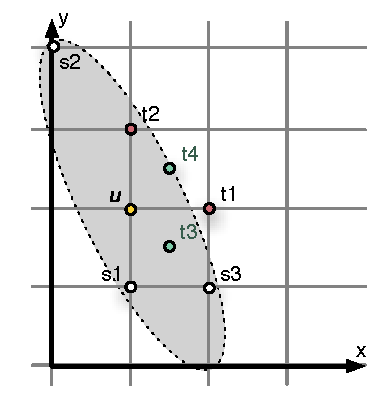
\includegraphics{points.pdf}
\begin{align*}
  \ve{t_1}  = & \begin{m} 2 & 2 \end{m} \\
  \ve{t_2}  = & \begin{m} 1 & 3 \end{m} \\
  \ve{\mu} = & \begin{m} 1 & 2 \end{m} \\
  \Sigma    = & \begin{m} 1 & -\frac{3}{2} \\ -\frac{3}{2} & 3\end{m}
\end{align*}

The \textbf{Euclidean distance} $d$ is the same for both points, even though it is visible that $\ve{t_1}$ is more ``out of the way" then $\ve{t_2}$ ~:
\begin{align*}
  d_1 = & \sqrt{\sum_{i=1}^{n}(t_i - \mu_i)^2} \\
     = & \sqrt{(2-1)^2 + (2-2)^2} = 1 \\
  d_2 = & \sqrt{(1-1)^2 + (3-2)^2} = 1
\end{align*}

The \textbf{normalized Euclidean distance} $d_{nE}$ should show that $\ve{t_2}$ matches the set $\ma{S}$ better then $\ve{t_1}$~:
\begin{align*}
  d_{1nE} = & \sqrt{\frac{(2-1)^2}{1} + \frac{(2-2)^2}{3}} = 1 \\
  d_{2nE} = & \sqrt{\frac{(1-1)^2}{1} + \frac{(3-2)^2}{3}} = \frac{1}{\sqrt{3}} \approx 0.6.
\end{align*}

This is better. We can see that $\ve{t_1}$ is penalized for being out of the way in the wrong direction. The ``penalty" for being badly adjusted along the $x$ axis is $1$ when it is only $\frac{1}{3}$ along the $y$ axis.

Let's now see what the Mahalanobis distance tells us. First we need to compute $\Sigma^{-1}$~:
\[
  \Sigma^{-1} = \frac{1}{(1*3 - -\frac{3}{2}*-\frac{3}{2})} \begin{m} 3 & \frac{3}{2} \\ \frac{3}{2} & 1\end{m} = \begin{m} 4 & 2 \\ 2 & \frac{4}{3} \end{m}
\]

We can now find the distances~:
\begin{align*}
  d_{1M} = & \sqrt{(\ve{t_1} - \ve{\mu})\Sigma^{-1}(\ve{t_1} - \ve{\mu})^T} \\
         = & \sqrt{\begin{m} 1 & 0 \end{m} \begin{m} 4 & 2 \\ 2 & \frac{4}{3}\end{m} \begin{m} 1 \\ 0 \end{m}} \\
         = & \sqrt{\begin{m} 4 & 2 \end{m} \begin{m} 1 \\ 0 \end{m}} = 2\\
  d_{2M} = & \sqrt{\begin{m} 0 & 1 \end{m} \begin{m} 4 & 2 \\ 2 & \frac{4}{3}\end{m} \begin{m} 0 \\ 1 \end{m}} \\
         = & \sqrt{\begin{m} 2 & \frac{4}{3}\end{m} \begin{m} 0 \\ 1 \end{m}} = \frac{2}{\sqrt{3}} \approx 1.2\\
\end{align*}

These distances classify the two vectors in the exactly the same way as the normalized Euclidean distances. Why is that so ? The reason is that our vectors are always away from the mean value in a single direction at a time, thus the ``covariance'' part of the error is never used.

What happens with the two points $\ve{t_3}$ and $\ve{t_4}$ ? From the first look at the picture we can see that their distance to the mean value is the same~:
\begin{align*}
  d_3 = & \frac{1}{\sqrt{2}} \approx 0.7 \\
  d_4 = & \frac{1}{\sqrt{2}} \approx 0.7
\end{align*}

Their normalized Euclidean values are also the same as they differ from the mean value exactly in the same way along $x$ and $y$~:
\begin{align*}
  d_{3nE} = & \frac{1}{\sqrt{3}} \approx 0.6\\
  d_{4nE} = & \frac{1}{\sqrt{3}} \approx 0.6
\end{align*}

Now comes the Mahalanobis distances~:
\begin{align*}
  d_{3M} = & \frac{1}{\sqrt{3}} \approx 0.6\\
  d_{4M} = & \frac{\sqrt{14}}{\sqrt{6}} \approx 1.5
\end{align*}

This type of distance calculation is the only one that reflect the difference between the two vectors $\ve{t_3}$ and $\ve{t_4}$ and classifies $\ve{t_4}$ as beeing further ``away'' then $\ve{t_3}$, like our eyes tell us from a quick look at the picture~!

\section{Eigenvalues}

Before we study \emph{Principal Component Analysis}, we need some understanding of eigenvalues. Imagine we have a transformation matrix $\ma{P}$~:
\[
  \ma{P} = \begin{m} 1 & 1 \\ 0 & 2 \end{m}.
\]

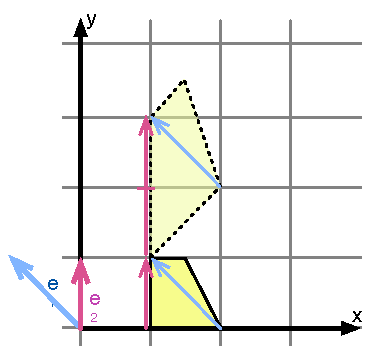
\includegraphics{eigen.pdf}

What are the vectors in this transformation that keep their direction (are not rotated) ? Mathematically speaking we want to find $\ve{e}$ such that~:
\[
  \ve{e'} = \ve{e} * \ma{P} = \lambda \ve{e}
\]

We can see from the picture that $\ve{y}$ satisfy this as $\ve{y'}$ is just $2 * \ve{y}$. Such vectors are called \emph{eigenvectors} and their corresponding lambda values \emph{eigenvalues}. To find these vectors, we can rewrite the equation above~:

\[
  \ve{e'} = \ve{e} * \ma{P} = \lambda \ve{e}
\]

as

\[
  \ve{e} * \ma{P} - \lambda \ve{e} = 0
\]

or 

\[
  \ve{e} (\ma{P} - \lambda \ma{I}) = 0  
\]

We know that an equation of the form~:
\[
  \ve{x} \ma{A} = 0
\]
has only the trivial solution $\ve{x} = \ve{0}$ if the determinant of $\ma{A}$ is not null. We can therefore find the non-trivial solutions to the equation above by computing the determinant when the latter \emph{is} null. This equation is called the \emph{characteristic equation} of $\ma{P}$~:
\[
  det(\ma{P} - \lambda \ma{I}) = 0
\]

We can now calculate the values of $\lambda$~:
\begin{align*}
  det(\begin{m} 1 & 1 \\ 0 & 2\end{m} - \lambda \begin{m} 1 & 0 \\ 0 & 1 \end{m}) = & 0 \\
  det(\begin{m} 1-\lambda & 1 \\ 0 & 2-\lambda\end{m}) = & 0 \\
  (1-\lambda)(2-\lambda) - 1 * 0 = & 0 \\
  (1-\lambda)(2-\lambda) = & 0
\end{align*}

which has the solutions
\[
\lambda_1 = 1, \lambda_2 = 2
\]

The corresponding \emph{eigenvectors} can be found by substituting $\lambda_1$ and $\lambda_2$ in $\ve{e} (\ma{P} - \lambda \ma{I}) = \ve{0}$~:
\begin{align*}
  \begin{m} x & y \end{m} \begin{m} 1-\lambda & 1 \\ 0 & 2-\lambda \end{m} = & 0 \\
  \begin{m} x_1 & y_1 \end{m} \begin{m} 1-1 & 1 \\ 0 & 2-1 \end{m} = & 0 \\
  \begin{m} x_1 & y_1 \end{m} \begin{m} 0 & 1 \\ 0 & 1 \end{m} = & 0 \\
  x_1 + y_1 = & 0 \\
  \ve{e_1} = & \begin{m} t & -t \end{m}
\end{align*}

and for $\lambda_2$~:
\begin{align*}
  \begin{m} x_2 & y_2 \end{m} \begin{m} 1-2 & 1 \\ 0 & 2-2 \end{m} = & 0 \\
  \begin{m} x_2 & y_2 \end{m} \begin{m} -1 & 1 \\ 0 & 0 \end{m} = & 0 \\
  -x_2  = & 0 \\
   x_2  = & 0 \\
  \ve{e_2} = \begin{m} 0 & t \end{m} = \ve{y}
\end{align*}

If we look at our transformation picture again, we see that the relation in the direction $\ve{e_1}$ is kept and the relation in the direction of $\ve{e_2}$ is just doubled. This reflects the eigenvalues $1$ and $2$ with the directions of the eigenvectors $\ve{e_1}$ and $\ve{e_2}$.


Before moving on to the following section, we need to establish some properties of \emph{symmetric} matrices. The first one is that such a matrix $\ma{A}$ can be expressed by the multiplication of a diagonal matrix $\ma{D}$ (all entries not on the diagonal are $\ve{0}$) and an invertible matrix $\ma{E}$~:
\begin{equation*}
  \ma{A} = \ma{E}^T\ma{D}\ma{E}. \label{symmetric}
\end{equation*}

Because $\ma{A}$ is symmetric, the transpose $\ma{A}^T$ of $\ma{A}$ (mirror across the diagonal) is the same as $\ma{A}$, we can therefore write~:
\begin{align*}
  \ma{A}^T = & (\ma{E}^T\ma{D}\ma{E})^T \\
           = &  \ma{E}^T(\ma{E}^T\ma{D})^T \\
           = &  \ma{E}^T\ma{D}^T\ma{E}^{TT}
\end{align*}
now we simply replace $\ma{D}^T$ by $\ma{D}$ since a diagonal matrix is equivalent to its transpose and we replace $\ma{E}^{TT}$ by $\ma{E}$ since transposing twice is equivalent to doing nothing. We get
\[
  \ma{A}^T = \ma{E}^T\ma{D}\ma{E} = \ma{A}.
\]

This proves that any matrix that can be expressed as a product of an invertible matrix $\ma{E}$ and a diagonal matrix $\ma{D}$ is indeed symmetric. We should now prove the reverse~: that any symmetric matrix can be expressed as stated above. This proof is called the \emph{spectral theorem}. While trying to understand it, I fell across strange names like \emph{Hermitian matrices}, \emph{Schur decomposition} and \emph{Hilbert spaces}. It also involved matrix calculations with complex numbers. That was too much me. Sorry. For those interested, I found a proof which you can consult on the web\footnote{(http://users.utu.fi/jkari/compression/kltaddition.pdf)}.

Anyway, let's pass on to the interesting part~: the matrix $\ma{E}$ used in the little talk above is in fact a matrix of the orthonormal eigenvectors of $\ma{A}$ (those vectors that do not rotate when transformed by $\ma{A}$). The proof is interesting but quite long, you can safely pass on to the section on \emph{Principal Component Analysis} if you do not have fun with letters in capital bold.

\emph{Please note that the following proofs are a rewrite of the first appendix of the tutorial on PCA by Jonathon Shlens\footnote{www.snl.salk.edu/~shlens/pub/notes/pca.pdf}}.

First, lets build this matrix $\ma{E}$ from the eigenvectors of $\ma{A}$~:
\[
  \ma{E} = \begin{m} \ve{e_1} \\ \vdots \\ \ve{e_n} \end{m}.
\]

Now let $\ma{D}$ be a diagonal matrix with the corresponding eigenvalues of $\ma{A}$~:
\[
  \ma{D} = \begin{m} \lambda_1 & 0 & .. \\ 0 & \lambda_2 & .. \\ \vdots & \vdots & \ddots \end{m}.
\]

We first try to prove that $\ma{E}\ma{A} = \ma{D}\ma{E}$~:
\begin{align*}
  \ma{E}\ma{A} = \begin{m} \ve{e_1} \\ \ve{e_2} \\ \vdots \end{m} \ma{A} = & 
                 \begin{m} \ve{e_1}\ma{A} \\ \ve{e_2}\ma{A} \\ \vdots \end{m} \\
  \ma{D}\ma{E} = \begin{m} \lambda_1 & 0 & .. \\ 0 & \lambda_2 & .. \\ \vdots & \vdots & \ddots \end{m} \ma{E} = & 
                 \begin{m} \lambda_1\ve{e_1} \\ \lambda_2\ve{e_2} \\ \vdots \end{m}.
\end{align*}

For $\ma{E}\ma{A}$ to be equal to $\ma{D}\ma{E}$, we must show that $\ve{e_i}\ma{A} = \lambda_i\ve{e_i}$ for all $i$. Remember that an eigenvector is \emph{a vector that is scaled onto itself by the transformation}, that is $\ve{e'} = \lambda\ve{e}$. This is exactly what the result of our equation states, thus the entries of $\ma{E}$ are the eigenvectors of $\ma{A}$ if $\ma{E}\ma{A} = \ma{D}\ma{E}$.

To finish the proof, we just need to show that $\ma{E}\ma{A} = \ma{D}\ma{E}$ implies $\ma{A} = \ma{E}^T\ma{D}\ma{E}$. By multiplying each side by $\ma{E}^{-1}$, we obtain $\ma{A} = \ma{E}^{-1}\ma{D}\ma{E}$. If we could show that $\ma{E}^{-1} = \ma{E}^T$, we would have proven (\ref{symmetric}). We know that $\ma{E}^{-1} = \ma{E}^T$ if $\ma{E}$ is an orthogonal matrix since~:
\begin{align*}
  \ma{E}\ma{E}^T = & \begin{m} \ve{e_1} \\ \ve{e_2} \\ \vdots \end{m} \begin{m} \ve{e_1}^T & \ve{e_2}^T & \hdots \end{m} \\
                 = & \begin{m} \ve{e_1}\ve{e_1}^T & \ve{e_1}\ve{e_2}^T & \hdots \\ \ve{e_2}\ve{e_1}^T & \ve{e_2}\ve{e_2}^T & \hdots \\ \vdots & \vdots & \ddots \end{m} \\
                 = & \begin{m} 1 & 0 & \hdots \\ 0 & 1 & \hdots \\ \vdots & \vdots & \ddots \end{m} \\
                 = & \ma{I}
\end{align*}

because each vectors in an orthogonal matrix is $\perp$ to other vectors, thus the dot product is zero except for the diagonal entries where it is equal to the squared norm of the vector. If we choose our eigenvectors so that their norm is 1, we obtain the identity matrix $\ma{I}$. We just need to show that $\ma{E}$ is an orthogonal matrix and pulling the thread out of this maze, we prove that a symmetric matrix can be expressed by (\ref{symmetric}). We want to know if $\vec(e_i) \dot \vec{e_j} = 0$ for all $i \not= j$. Let $\lambda_i$ and $\lambda_j$ be two distinct eigenvalues.
\begin{align*}
  \lambda_i\ve{e_i} \cdot \ve{e_j} = & \lambda_i\ve{e_i}\ve{e_j}^T \\
                                  = & \ve{e_i}\ma{A}\ve{e_j}^T \\
                                  = & \ve{e_i}(\ve{e_j}\ma{A}^T)^T \\
                                  = & \ve{e_i}(\ve{e_j}\ma{A})^T \\
                                  = & \ve{e_i}(\lambda_j\ve{e_j}^T) \\
  \lambda_i\ve{e_i} \cdot \ve{e_j} = & \ve{e_i} \cdot \lambda_j\ve{e_j}
\end{align*}

Thus $(\lambda_i - \lambda_j)\ve{e_i} \cdot \ve{e_j} = 0$. Since we have conjectured that $\lambda_i \not= \lambda_j$, it must be that $\ve{e_i}$ and $\ve{e_j}$ are orthonormal (their dot product is $0$). Therefore $\ma{E}^{-1} = \ma{E}^T$ and we can write~:
\[
  \ma{A} = \ma{E}^T\ma{D}\ma{E}.
\]

All this work, just to reexpress an arbitrary symmetric matrix $\ma{A}$\dots But this result is the ground on which the next section is built.

\section{Principal Component Analysis}

Principal Component Analysis is a way to extract the ``most proeminent features'' of a data set. It assumes that the data has a good signal to noise ratio which means that \emph{great variance} in the data is a synonym for \emph{relevant feature} and not \emph{big noise}.

In all the calculations below, we need to use the \emph{variations} of the measures. We will thus remove the mean values from our data set and use this new set called the \emph{mean deviation form} of $\ma{S}$~:
\[
  \ma{T} = \ma{S} - \begin{m}\ve{\mu} \\ \vdots \\ \ve{\mu}\end{m}.
\]

In order to extract the ``most proeminent features'' of our data, a good idea would be to look at the directions in which the data varies most. Is it along the $\ve{x}$ axis ? The $\ve{y}$ axis ? Somewhere in between ?

Recall from the previous sections that the variance-covariance matrix $\ma\Sigma$ displays variances along the diagonal and covariances off-diagonal. We can use this matrix to extract directions in which the data varies most~:
\[
  \ma\Sigma = \frac{1}{n-1}\ma{T}^T\ma{T}.
\]

By looking at the diagonals of $\Sigma$, we pick the greatest absolute value and there we are, we found our direction ($3 \Rightarrow \ve{y}$). Is that it ? No, this solution misses the fact that the main direction might not follow one of the axis (dimension) of our recorded data (the ellipsoid is not vertical nor horizontal). What we need is to apply a transformation (rotation + stretch) to our data $\ma{T}$ into an new basis $\ma{P}$ prior to looking at the variance-covariance matrix, so that the principal components align with the new basis' axis.
\begin{align*}
  \ma{T'} = & \ma{T}\ma{P} \\
  \ma\Sigma'     = & \frac{1}{n-1}\ma{T'}^T\ma{T'}
\end{align*}

Our goal is thus to find a new basis $\ma{P}$ that gives us great absolute values along the diagonals of $\ma\Sigma'$ and small absolute values off-diagonal (small redundancy). If possible, it would be great to see large variances along the top of the diagonal which would mean we could just cut off the rightmost part of the matrix $\ma{T'}$ and still have most of the information on the varying signal. To summarize~:
\begin{itemize}
  \item Find a new basis $\ma{P}$ that reduces the redundancy of the signals (low covariance).
  \item The $\ma\Sigma'$ matrix for $\ma{T'}$ should ideally be a diagonal matrix with very high values at the top and very small at the bottom, thus showing signals in the first dimensions and pure noise in the last ones.
  \item We could then choose to remove the columns of $\ma{T'}$ that have greater indices than the number of dimensions we want to keep thus reducing the dimensionality of our data.
\end{itemize}

A simple way to find the solution would be~:
\begin{enumerate}
  \item Find the direction $\ve{e_1}$ that shows the greatest variance in the data $\ma{T}$. Normalize this vector. This is our first basis vector.
  \item Find another normalized vector showing the greatest variance that is orthogonal to those already found ($\forall \ve{b}\in \{\text{found vectors}\}, \ve{e_n} \perp \ve{b}$).
  \item Repeat until we have $n$ basis vectors ($n$ is the size of vector space).
\end{enumerate}

The resulting ordered set of vectors are the \emph{principal components} of our data set \textbf{T}.

\section{computing PCA}

Mathematically stated, what we are looking for is a diagonalized version of $\ma\Sigma'$~:
\begin{align*}
  \ma\Sigma'     = & \frac{1}{n-1}\ma{T'}^T\ma{T'} \\
                 = & \frac{1}{n-1}(\ma{T}\ma{P})^T(\ma{T}\ma{P}) \\
                 = & \frac{1}{n-1}\ma{P}^T\ma{T}^T\ma{T}\ma{P}
\end{align*}

Does this look familiar to you ? Recall all our lengthy discussion on symmetrical matrices ? Well, $\ma{T}^T\ma{T}$ is such a matrix. Lets replace it by $\ma{A}$. We get~:
\[
  \ma\Sigma'     = \frac{1}{n-1} \ma{P}^T\ma{A}\ma{P}
\]

Now what happens if we set $\ma{P} = \ma{E}^T$ and replace $\ma{A}$ by $\ma{E}^T\ma{D}\ma{E}$ from equation (\ref{symmetric}) ?
\begin{align*}
  \ma\Sigma' = & \frac{1}{n-1}\ma{E}\ma{A}\ma{E}^T \\
             = & \frac{1}{n-1}\ma{E}(\ma{E}^T\ma{D}\ma{E})\ma{E}^T \\
             = & \frac{1}{n-1}\ma{I}\ma{D}\ma{I} \\
             = & \frac{1}{n-1}\ma{D}
\end{align*}

We have just found the transformation that diagonalizes the variance-covariance matrix. It's the transpose of the matrix of eigenvectors of $\ma{T}^T\ma{T}$ !
\[
  \ma{P} = \ma{E}^T = \begin{m} \ve{e_1}^T & \ve{e_2}^T & \hdots \end{m}
\]
where $\ve{e_i}$ is $i$th eigenvector of $\ma{T}^T\ma{T}$.

\section{applying PCA to $\ma{S}$}

Using the same sample data as above, we imagine that the set of points $\textbf{S}$ represents the measures of a moving element. The object actually moves only along the ellipsoid axis $\ve{e} = \begin{m}-1 & 2 \end{m}$, the deviations from this axis is just noise. The goal of PCA is to re-express our set of data in a new basis that reflects this behaviour (data along $\ve{e}$, noise along the other direction). The naive basis (in which we recorded the data) is~:
\[
  \ma{B} = \begin{m} \ve{x} \\ \ve{y} \end{m} = \begin{m} 1 & 0 \\ 0 & 1 \end{m} = \ma{I}
\]

We will use PCA to find a new basis $\ma{P}$ that is a linear combination of the original basis $\ma{B}$ and in which we will only look at the data along the greatest axis of the ellipsoid (where the data exhibits the greatest variance). In this new basis, the set of data $\ma{S}$ becomes~:
\[
  \ma{S'} = \ma{S}\ma{P}
\]

The new basis should optimise signal to noise ratio if we consider the first dimension as representing the signal and the second the noise~:
\[
  SNR = \frac{\sigma_{signal}^2}{\sigma_{noise}^2}
\]

Before delving any further, we must first transform our data into its \emph{mean deviation form} $\ma{T}$. 
\[
  \ma{T} = \ma{S} - \begin{m}\ve{\mu} \\ \vdots \\ \ve{\mu}\end{m} = \begin{m} 0 & -1 \\ -1 & 2 \\ 1 & -1\end{m}.
\]

We can now easily compute the actual SNR~:
\[
  SNR = \frac{\sum_{k=1}^l T_{k1}^2}{\sum_{k=1}^l T_{k2}^2} = \frac{0+1+1}{1+4+1} = \frac{1}{3}
\]

How do we find the new basis that gives us the greatest SNR ? Expressed in another way, we could say~: how do we find the basis that shows greatest variance in the first dimension and mostly noise in the second ? From the preceding section, we know how to build $\ma{P}$. Let's do it with our data. First we need to find the symmetric matrix $\ma{A}$~:
\begin{align*}
  \ma{A} = & \ma{T}^T\ma{T} = \begin{m} 0 & -1 & 1 \\ -1 & 2 & -1 \end{m} \begin{m} 0 & -1 \\ -1 & 2 \\ 1 & -1\end{m} \\
         = & \begin{m} 2 & -3 \\ -3 & 6 \end{m}
\end{align*}

Now we must find the eigenvalues of this matrix~:
\begin{align*}
  det(\ma{A} - \lambda\ma{I}) = & 0 \\
  det(\begin{m} 2-\lambda & -3 \\ -3 & 6-\lambda \end{m}) = & 0 \\
  (2-\lambda)(6-\lambda) - 9 = & 0 \\
  \lambda^2 - 8\lambda + 3 = & 0 \\
  \lambda_1 \approx 7.6, \lambda_2 \approx 0.4.
\end{align*}

The corresponding eigenvectors are~:

\begin{align*}
  \begin{m}x & y\end{m}\begin{m} 2-\lambda & -3 \\ -3 & 6-\lambda \end{m} = & 0 \\
  \left\{ \begin{array}{rl} x = & \frac{3}{2-\lambda} t \\ y = & t \end{array} \right.
\end{align*}

We want normed vectors so we add the rule $x^2 + y^2 = 1$ and we get~:
\begin{align*}
  \frac{9t^2}{(2 - \lambda)^2} + t^2 = & 1 \\
  t = & \frac{2-\lambda}{\sqrt{9 + (2 - \lambda)^2}} \\
  t_1 \approx & -0.9 \\
  t_2 \approx & 0.5 \\
  \ma{E} \approx & \begin{m}0.5 & -0.9 \\ 0.9 & 0.5 \end{m}.
\end{align*}

Now that we have our transformation matrix $\ma{P}$
\[
  \ma{P} = \ma{E}^T = \begin{m}0.5 & 0.9 \\ -0.9 & 0.5 \end{m}.
\]
we can transform our data $\ma{T}$ into $\ma{T}'$~:
\begin{align*}
  \ma{T}' = & \ma{T}\ma{P} \approx \begin{m} 0 & -1 \\ -1 & 2 \\ 1 & -1\end{m}\begin{m}0.5 & 0.9 \\ -0.9 & 0.5 \end{m} \\
    \approx & \begin{m} 0.9 & -0.5 \\ -2.2 & 0.1 \\ 1.4 & 0.4 \\ \end{m}
\end{align*}

With this new transformation, we should have great variance along the first dimension and a very small one in the second (that was our goal). By looking at the values, this seems to be the case. Let's see with a picture.

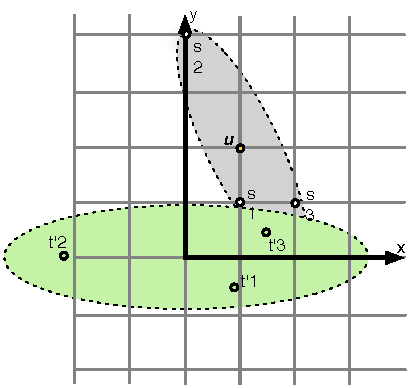
\includegraphics{points2.pdf}

Just to make sure our work was correct, let's compute the variance-covariance matrix $\ma\Sigma'$~:
\[
  \ma\Sigma' = \frac{1}{n-1}\ma{T'}^T\ma{T'} \approx \begin{m} 7.6 & 0 \\ 0 & 0.4 \end{m}.
\]

It works ! And by the way, this is $\ma{D}$ which is the diagonal matrix made out of the eigenvalues of $\ma{A} = \ma{T}^T\ma{T}$ ($7.6$ and $0.4$).

To finish our goal of dimensionality reduction, we can build another version of the matrix $\ma{P}$ that automatically strips off the ``noisy'' dimensions, only keeping the principal components of our data~:
\[
  \ma{Q} = \ma{P}\begin{m} 1 \\ 0 \end{m} = \begin{m}0.5 \\ -0.9\end{m}.
\]

And before closing this section, we need to compute our new signal to noise ratio~:
\[
  SNR = \frac{\sum_{k=1}^l {T'}_{k1}^2}{\sum_{k=1}^l {T'}_{k2}^2} \approx \frac{7.6}{0.4} = 19.3.
\]

By just looking at the $\ve{y}$ axis, we would have obtained $3$. Applying the transformation $\ma{P}$ made the signal much easier to analyse.

That's it (I'm glad I made it this far) !

\subsection{summary on PCA}

PCA can be used as a filter to reduce the dimensionality of the data and ease the computation of the \textbf{Mahalanobis distance} as this distance becomes the \textbf{normalized Euclidean distance} with the new transformation since the covariances have been removed ($\ma\Sigma'$ is a diagonal matrix). The calculation of the transformation matrix $\ma{P}$ involves the following computations~:
\begin{itemize}
  \item Find the mean vector $\ve\mu$.
  \item Substract this vector to each vector of the training set $\ma{S}$ to obtain the \emph{mean deviation form} $\ma{T}$.
  \item Find the eigenvectors of the symmetric matrix $\ma{T}^T\ma{T}$, sorted by decreasing eigenvalues.
  \item Build the transformation matrix $\ma{P} = \begin{m}\ve{e_1}^T & \ve{e_2}^T & \hdots & \ve{e_k}^T \end{m}$ with $k \leq n$ to keep the $k$ most relevant dimensions of the transformed data.
  \item Apply this transformation $\ma{P}$ to any test vector $\ve{t}$ before computing the normalized Euclidean distance to the mean value $\ve\mu$.
  \item The smaller the distance, the bigger the probability that $\ve{t}$ belongs to the set $\ma{S}$.
\end{itemize}

Among all the steps above, two are problematic for large matrices: finding the eigenvalues and eigenvectors. These steps imply solving the \emph{characteristic polynomial} of $\ma{A}$. If our data contains 12 measures x 100 samples per row, the dimension of our polynomial is 1200 ! To find the eigenvector we have to solve n times a system of n-1 equations. This can become daunting. That was for the bad news. The good news is that these calculations must only be done on the training set, not live. The even better news is that there exists a library written in Fortran called \emph{LAPACK} that can do the job as fast as the most clever people could make it. Thanks.
\subsection{notes on PCA}

For a deaper understanding of PCA and it's limits, one may have a look at~:
\begin{itemize}
  \item \emph{kernel PCA} to apply a non-linear filter prior to applying PCA for problems where linearity is an issue.
  \item \emph{ICA} for sets of data whose distribution probabilities are not exponential (Gaussian, Exponential, etc).
  \item \emph{Central Limit Theorem} on why PCA should work most of the time in real world as probabilities usually \textbf{are} gaussian.
\end{itemize}


\section{Movement recognition}

From the knowledge we have gathered above, we can now try to find a way to compare the movements. Imagine we have 3 movements (classes) labeled $a$, $b$ and $c$. Each movement has been recorded several times. We create the training sets $\ma{S_a}$, $\ma{S_b}$ and $\ma{S_c}$ with the recordings of the different movements. Each move is made of 2 measures recorded for 10 samples. We write it as a row vector of dimension 20 ($\ve{s_{ai}}$).


\section{Filtering (PCA)}

We start by computing the mean vector for each movement. We will note the number of recordings for the current movement $r$~:
\[
  \ve\mu_a = \frac{1}{r}\sum_{k=1}^r \begin{m}\ve{s_{a1k}} & \ve{s_{a2k}} & \hdots & \ve{s_{a20k}} \end{m}
\]
We do this for each class $a$, $b$ and $c$. We then build a matrix out of these prototypes~:
\[
  \ma{S} = \begin{m}\ve\mu_a \\ \ve\mu_b \\ \ve\mu_c \end{m}
\]

We now find the mean deviation form of $\ma{S}$ after finding the mean value of all the prototypes ($\ve\mu$)~:
\[
  \ma{T} = \begin{m}\ve\mu_a - \ve\mu \\ \ve\mu_b - \ve\mu \\ \ve\mu_c - \ve\mu \end{m}
\]

Now that we have found the \emph{least varying parts} of each movement (the ``platonic idea'') by computing the average, we will find a transformation that shows the \emph{most varying parts} \textbf{between} these movements. We apply PCA on the matrix $\ma{T}$ and find the transformation matrix $\ma{P}$.
\[
  \ma{P} = \ma{E}^T \ma{I_{reduc}}
\]
Where $\ma{I_{reduc}}$ is a truncated identity matrix to reduce the dimensionality of the data to the principal components.

\section{Recognition}

To label new vectors, we could use the Mahalanobis distance or Euclidean distance in the transformed vector space produced by PCA. This is the first solution discussed below. The other approach is to use \emph{Support Vector Machines}. This is the solution which we will try to use if our hardware is fast enough since it produces better results.

\subsection{Distances}

We now have two options. Either we use the information contained in the eigenvalues (matrix $\ma{D}$) to compute the normalized Euclidean distances between our test vector and the prototypes in the new coordinate system defined by the transformation $\ma{P}$ or we map all our training data into the new coordinate system and compute the Mahalanobis distance to each set. This last solution loses some information from the \emph{differences between the different classes $a$, $b$ and $c$} but takes into account what is noise and what is a signal in each movement. Since we have already included the information on what makes the differences between the classes when we chose to remove the dimensions with least variance, the second solution seems to keep most of the information contained in the training data.

Transforming each training set into the new coordinate system is done by
\begin{align*}
  \ma{S_{a}'} = & \ma{S_a}\ma{P} \\
  \ma{S_{b}'} = & \ma{S_b}\ma{P} \\
  \ma{S_{c}'} = & \ma{S_c}\ma{P} \\
\end{align*}

We now compute the variance-covariance for each of these matrices~:
\begin{align*}
  \ma\Sigma_a' = & \frac{1}{r-1}\ma{S_{a}'}^T\ma{S_{a}'} \\
  \ma\Sigma_b' = & \frac{1}{r-1}\ma{S_{b}'}^T\ma{S_{b}'} \\
  \ma\Sigma_c' = & \frac{1}{r-1}\ma{S_{c}'}^T\ma{S_{c}'} \\
\end{align*}

Normalization of the values in these matrices ?
\begin{align*}
  \ma\Sigma_{aij}' = & \frac{\ma\Sigma_{aij}'}{\sum_{k=1}^3 \ma\Sigma_{kij}'}
\end{align*}

To label an arbitrary movement $\ve{t}$, we find the minimal Mahalanobis distance to the sets in the new coordinate system.
\begin{align*}
  \ve{t_k'} = & \ve{t'} - \ve{\mu_k'} \\
            = & \ve{t}\ma{P} - \ve{\mu_k'} \\
  \argmin_{k} D_M(\ve{t}) = & \argmin_{k} \sqrt{\ve{t_k'}\Sigma_k'^{-1}\ve{t_k'}^T}
\end{align*}

The value returned by argmin ($k$) is the label for the test movement.

\subsection{Support Vector Machines}

\emph{Support Vector Machines} is a new mathematical tool for pattern recognition. Basically, it involves mapping the data into a new vector space (once more) with higher dimensions this time. The goal is to find a vector space in which the data is linearly separable (you can draw a line/plane/... between the different classes). For example, imagine you have two sets of data $a$ and $b$: all values for set $a$ are inside a circle located on the origine and all values for $b$ are outside of this circle. If we add a third dimension that is the distance to the origine, we will obtain a cone pointing downward. All points from the set $a$ are located below a certain height and all point from set $b$ are above this height. We can thus split the set using a plane that cuts the cone at this height.

To apply SVM, we first filter all our data set with PCA:
\begin{align*}
  \ma{S_{a}'} = & \ma{S_a}\ma{P} \\
  \ma{S_{b}'} = & \ma{S_b}\ma{P} \\
  \ma{S_{c}'} = & \ma{S_c}\ma{P} \\
\end{align*}

We then feed the svm library\footnote{http://www.csie.ntu.edu.tw/~cjlin/libsvm} (we could never have written this code) with two arrays~: a list of labels and a list of vectors. We thus feed it with set $S_{a}'$, telling it these vectors have the label ``a'', $S_{b}'$ with label ``b'' and $S_{c}'$ with label ``c''. We then call the learn function.

To test an arbitrary movement $\ve{t}$, we must first move it into the vector space defined by PCA and then send it into SVM. The SVM black box will return the label for the test vector.
\begin{align*}
  \ve{t_k'} = & \ve{t'} - \ve{\mu_k'} \\
            = & \ve{t}\ma{P} - \ve{\mu_k'} \\
  \text{label} = & \text{svmlib.predict}(\ve{t_k'})
\end{align*}

\onecolumn

\section{Ruby code}
\subsection{variance}
\begin{verbatim}
set   = [1,4,3,6]
mu    = set.inject(0) {|s,v| s + v } / set.size.to_f
sigma = set.inject(0) {|s,v| s + ((v - mu)**2) } / set.size.to_f
\end{verbatim}

\subsection{Mahalanobis distance}
\begin{verbatim}
class Array
  # transpose
  def t
    cols = []
    self[0].each_index do |i|
      cols[i] = map {|v| v[i]}
    end
    cols
  end

  def *(m)
    res = []
    each_index do |row|
      res[row] = []
      m[0].each_index do |col|
        res[row][col] = 0
        self[0].each_index do |i|
          res[row][col] += self[row][i] * m[i][col]
        end
      end
    end
    res
  end

  def det
    (self[0][0] * self[1][1]) - (self[1][0] * self[0][1])
  end

  def /(scalar)
    map {|row| row.map {|v| v / scalar}}
  end

  # vector substraction
  def -(v)
    res = [[]]
    self[0].each_index {|i| res[0][i] = self[0][i] - v[0][i]}
    res
  end

  def to_s
    if self.size > 1 || self[0].size > 1
      if self.size == 1
        row_format = '[' + (" %3.1f" * self[0].size) + " ]\n"
      else
        row_format = '|' + (" %3.1f" * self[0].size) + " |\n"
      end
      self.inject("") {|s,row| s + sprintf(row_format, *row)}
    else
      self[0][0].to_s
    end
  end

  def map_index(&block)
    res = []
    self.each_index do |i|
      res[i] = yield(i,self[i])
    end
    res
  end
end


set = [[1,1],
       [0,4],
       [2,1]]
# mean vector mu
mu = [[]]
set[0].each_index do |i|
  mu[0][i] = set.inject(0) {|s,v| s + v[i] } / set.size.to_f
end

# set - mu
s_mu = set.map do |v|
  r = []
  v.each_index do |i|
    r[i] = v[i] - mu[0][i]
  end
  r
end

# variance-covariance matrix
sigma = (s_mu.t * s_mu) / (set.size - 1.0).to_f

# inverse of sigma
if sigma.det == 0
  puts "Matrix not invertible"
  return
end

# invers of sigma (only for a 2x2 matrix)
sigma_inv = [[  sigma[1][1], -sigma[0][1] ],
             [ -sigma[1][0],  sigma[0][0] ]] / sigma.det

puts "Sigma\n\n"
puts sigma.to_s
puts "\nSigma's inverse\n\n"
puts sigma_inv.to_s

puts "\n\nAll results express value^2 (before square root)"

[
[[[2  , 2  ]],
[ [1  , 3  ]]],
[[[1.5, 1.5]],
[ [1.5, 2.5]]]
].each do |t1,t2|
  puts "\n-----------------------------"
  puts "t1   = #{t1}"
  puts "t2   = #{t2}"
  puts "t1-u = #{t1 - mu}"
  puts "t2-u = #{t2 - mu}\n\n"

  d1 = (t1 - mu).flatten.inject(0) {|s,v| s + v**2} 
  d2 = (t2 - mu).flatten.inject(0) {|s,v| s + v**2}

  puts "d1   = #{d1}"
  puts "d2   = #{d2}\n\n"

  d1nE = (t1 - mu).flatten.map_index{|i,v| v**2 / sigma[i][i] }.inject(0) {|s,v| s + v } 
  d2nE = (t2 - mu).flatten.map_index{|i,v| v**2 / sigma[i][i] }.inject(0) {|s,v| s + v } 

  puts "d1nE = #{d1nE}"
  puts "d2nE = #{d2nE}\n\n"

  d1M = (t1 - mu) * sigma_inv * (t1 - mu).t
  d2M = (t2 - mu) * sigma_inv * (t2 - mu).t

  puts "d1M  = #{d1M}"
  puts "d2M  = #{d2M}\n\n"
end
\end{verbatim}
\end{document}